\PassOptionsToPackage{dvipsnames}{xcolor}
\PassOptionsToPackage{usenames}{color}
\documentclass{beamer}[10]
%\usepackage{pgf}
\usepackage[english]{babel}
\usepackage[utf8]{inputenc}
\usepackage{amsmath,amsfonts,amssymb,wasysym}
\usepackage{beamerthemesplit}
\usepackage{graphics,epsfig}
\usepackage{caption}
\usepackage{subcaption}
\usepackage{url}
\usepackage{srcltx}
\usepackage{hyperref}
\usepackage{media9,graphicx}
\usepackage{multicol}
\usepackage{adjustbox}
\usepackage{natbib}
\usepackage{appendixnumberbeamer}
\setlength{\bibsep}{4pt}
\renewcommand{\arraystretch}{1.3}
\graphicspath{{../Figures/}{../../Figures/}}

\usepackage{tikz}
\usetikzlibrary{shapes.geometric, arrows}
\tikzstyle{startstop} = [rectangle, rounded corners, minimum width=3cm, minimum height=1cm,text centered, draw=black, fill=red!30]
\tikzstyle{io} = [trapezium, trapezium left angle=75, trapezium right angle=105, minimum width=2cm, minimum height=1cm, text centered, draw=black, fill=blue!30]
\tikzstyle{process} = [rectangle, minimum width=3cm, minimum height=1cm, text centered, draw=black, fill=orange!30]
\tikzstyle{decision} = [rectangle,, rounded corners, minimum width=3.5cm, minimum height=1.5cm, text centered, draw=black, fill=green!30]
\tikzstyle{arrow} = [thick,->,>=stealth]
%\renewcommand*{\bibfont}{\footnotesize}
\setbeamertemplate{footline}[frame number]
%\setbeamerfont{bibliography item}{size=\footnotesize}
%\setbeamerfont{bibliography entry author}{size=\footnotesize}
%\setbeamerfont{bibliography entry title}{size=\footnotesize}
%\setbeamerfont{bibliography entry location}{size=\footnotesize}
%\setbeamerfont{bibliography entry note}{size=\footnotesize}

\definecolor{kugreen}{RGB}{50,93,61}
\definecolor{kugreenlys}{RGB}{132,158,139}
\definecolor{kugreenlyslys}{RGB}{173,190,177}
\definecolor{kugreenlyslyslys}{RGB}{214,223,216}

\setbeamerfont{caption}{size=\tiny}
\setbeamercovered{transparent}
\mode<presentation>{}
\usetheme[numbers,totalnumber, compress,sidebarshades]{PaloAlto}


\usecolortheme[named=kugreen]{structure}
\useinnertheme{circles}
\usefonttheme[onlymath]{serif}
\setbeamercovered{transparent}
\setbeamertemplate{blocks}[rounded][shadow=true]


\useoutertheme{smoothbars} 

%\AtBeginSection[]
%{
%	\begin{frame}
%		\frametitle{Table of Contents}
%		\tableofcontents[currentsection]
%	\end{frame}
%}

\AtBeginSubsection[]{
	\begin{frame}[noframenumbering]
		\frametitle{Table of Contents}
		\begin{multicols}{2}
			\tableofcontents[currentsubsection]
		\end{multicols}
	\end{frame}
}

%\AtBeginSection[]{
%	\begin{frame}
%		\frametitle{Table of Contents}
%		\begin{multicols}{2}
%			\tableofcontents[currentsection]
%		\end{multicols}
%	\end{frame}
%}

\title{Laki to Tambora}
%\author{Thea Quistgaard}
\subtitle{\small \textit{Signal Restoration and Pattern Recognition in Ultra High Resolution Volcanic and Isotopic Signals}}
\author[T. Quistgaard]{Thea Quistgaard\\[1ex]  {\small Supervisors: Vasileios Gkinis \& James Avery}}
%\author{Supervisor: V. Gkinis \& J. Avery}
\institute[UCPH]{University of Copenhagen}
\logo{\includegraphics[width=0.8cm]{KULogo-eps-converted-to.pdf}}

\begin{document}
	{\setbeamertemplate{footline}[frame number]
		\frame{\titlepage \vspace{-0.5cm}	
	}}
	
	\begin{frame}{Laki to Tambora}
		\begin{figure}[h]
			\centering
			\includegraphics[width=0.8\textwidth]{TurnerEruptionofSoufriere-Mountains.jpg}
			\caption{J. M. W. Turner: \textit{The Eruption of the Soufriere Mountains in the Island of St Vincent, 30 April 1812}, 1815}
		\end{figure}
	\end{frame}
	
	\begin{frame}{Outline}
		\setcounter{tocdepth}{1}
			\tableofcontents
		
	\end{frame}
	\setcounter{tocdepth}{2}	
	
	%\setbeamertemplate{footline}[frame number]
	\addtocounter{page}{-1}
	
	
	
	
	
	
	
	\section[Introduction]{Introduction}
	\subsection{Basic Problem}
	\frame{
		\frametitle{Water Isotopes in Greenlandic Ice Cores}
		\begin{center}
			$\delta^{18}\text{O} = \frac{^{18}R_{sample}}{^{18}R_{reference}} - 1$, where $^{18}R = \frac{n_{^{18}\text{O}}}{n_{^{16}\text{O}}}$
		\end{center}
			
			
				\begin{figure}[h]
					\centering
					\includegraphics[width=0.45\textwidth]{FractionationDrawing.pdf}
					\caption{Fractionation through evaporation, transportation and precipitation along with typical water isotopic ratios in [\permil]}
					\label{Fig:FractionationDrawing}
				\end{figure}
	}

	\frame{
		\frametitle{Water Isotopes in Greenlandic Ice Cores: Crête}
		
			\begin{figure}[h]
				\centering
				\includegraphics[width=\textwidth]{Crete_10m_dated.pdf}
				\caption{Ten meters of the top of Cretê ice core, with identification and dating of 19 annual layers. Dating as from \url{https://www.iceandclimate.nbi.ku.dk/research/strat_dating/annual_layer_count/ice_core_dating/}}
				\label{Fig:ICE_Crete_10m_dated}
			\end{figure}
	}
	\frame{
		\frametitle{Water Isotopes in Greenlandic Ice Cores: Diffusion´}
		\begin{figure}[h]
			\centering
			\includegraphics[width=\textwidth]{Crete_first100m.pdf}
			\caption{100 meters of the Crête ice core, with diffusion visible.}
			\label{Fig:Crete_100m}
		\end{figure}
		
		\begin{itemize}[<+->]
			\item Diffusion: Displacement of water isotopes in the firn column
			\item \textbf{Parameter of interest}: Diffusion length, $\sigma$
			\item $\sigma$ dependent on temperature $T$
		\end{itemize}
	}

	\frame{
		\frametitle{Ice Cores in this Project}
		\only<1>{
			\begin{figure}
				\centering
				\includegraphics[width=0.5\textwidth]{AlphabetCores1.pdf}
				\caption[Map of Greenlandic ice core locations]{Location of Alphabet cores along with some major ice cores, NEEM, EGRIP and NGRIP.}
				\label{Fig:AlphabetCoresMap}
			\end{figure}
		}
		\only<2>{
			\begin{figure}[!htb]
				\centering
				\includegraphics[width=0.85\textwidth]{AlphabetCores1_Zoom.pdf}
				\caption[Alphabet Cores Map]{Map of spatial locations of the shallow Alphabet cores and deep core Crête analyzed in this thesis.}
				\label{Fig:MapAlphabetCores}
			\end{figure}
		}
	}

	\frame{
		\frametitle{A Rare Gem of Knowledge}
		\only<1>{
		\begin{figure}[h]
			\centering
			\includegraphics[width=\textwidth]{SiteA_ECM_d18O_full.pdf}
			\caption{Site A, full $\delta^{18}$O and ECM data series.}
			\label{Fig:SiteA_ECM_d18O_full}
		\end{figure}
		}
		\only<2>{
			\begin{figure}[h]
				\centering
				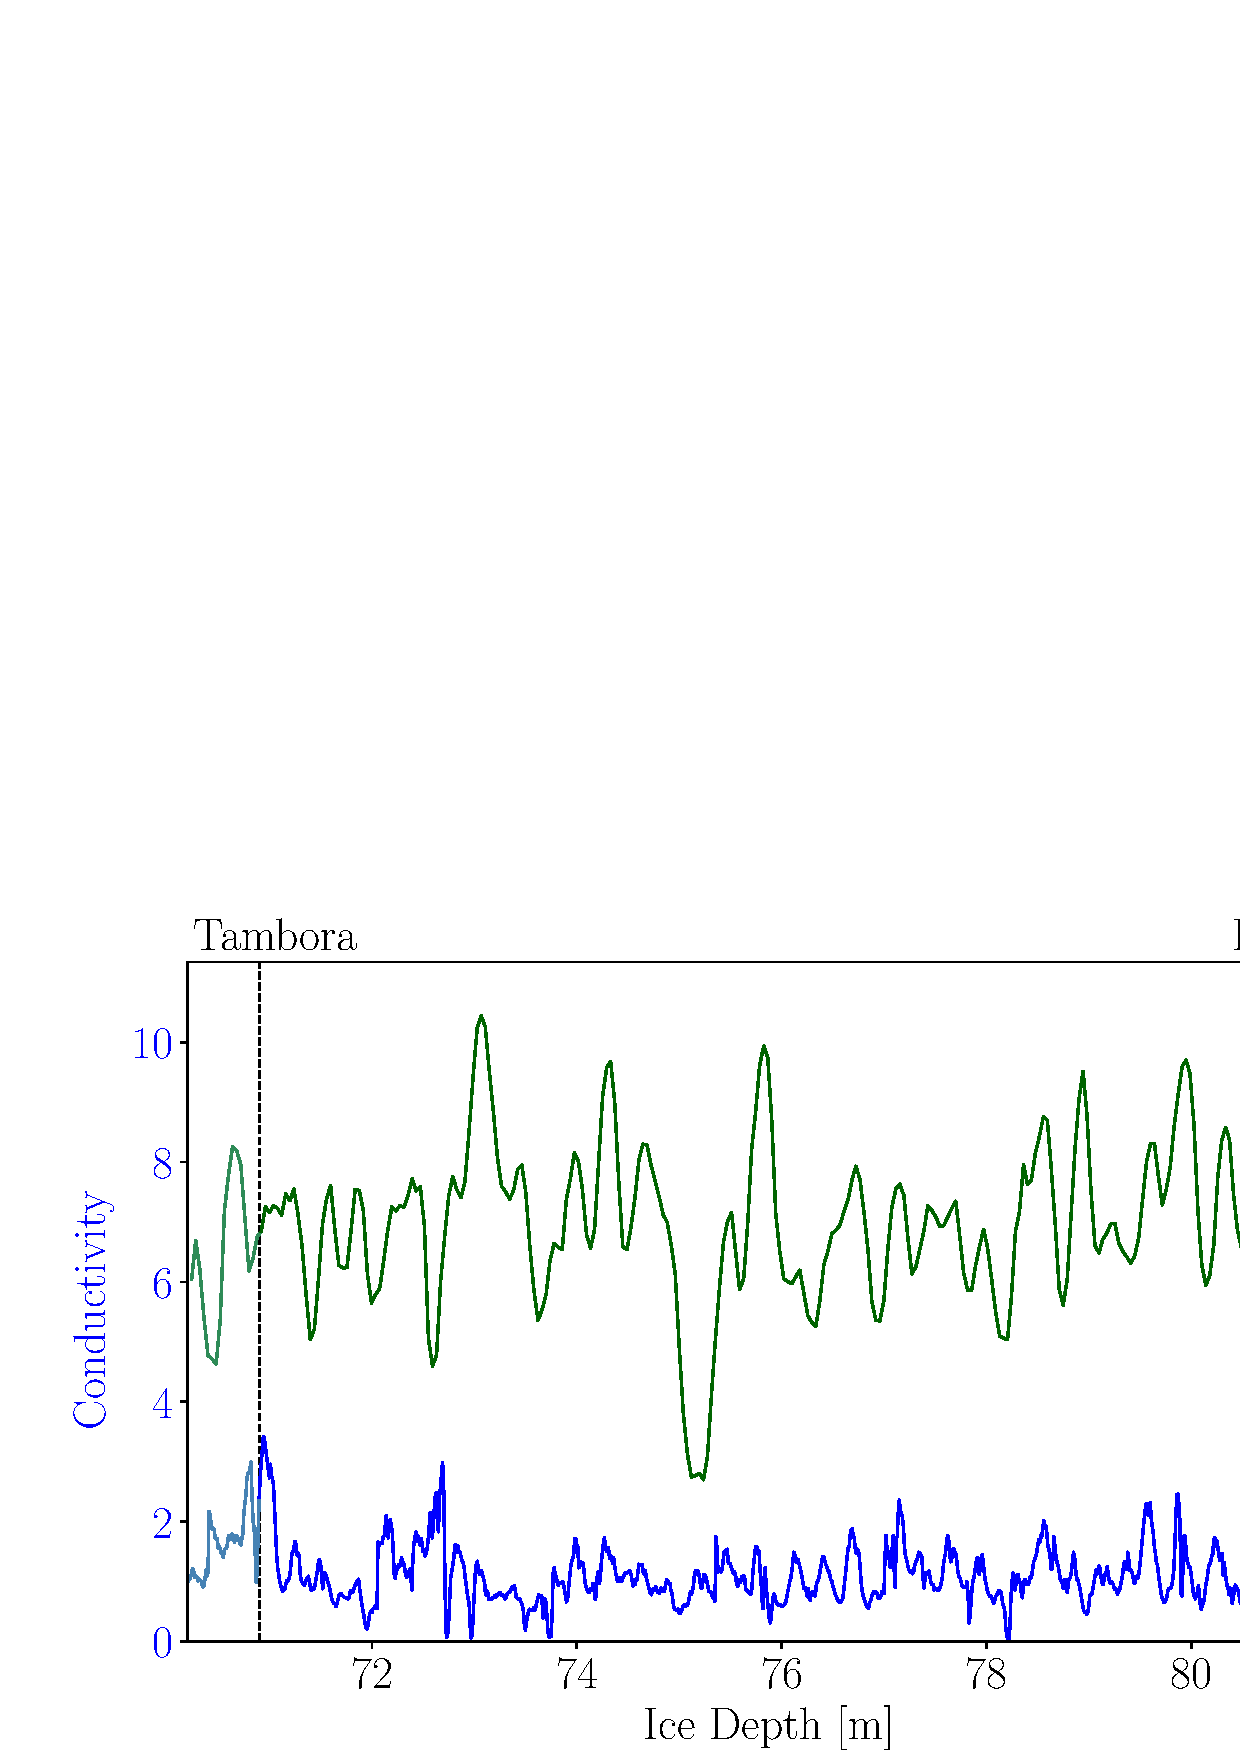
\includegraphics[width=\textwidth]{SiteA_ECMd18O_combo.pdf}
				\caption{Site A, Laki to Tambora $\delta^{18}$O and ECM data series.}
				\label{Fig:SiteA_ECMd18O_combo}
			\end{figure}
		}
	}
	
	\subsection[Goal]{Goal}
	

	\frame{
		\frametitle{Goal and Objective}
		
			\begin{adjustbox}{max totalsize={.9\textwidth}{.7\textheight},center}

			\begin{tikzpicture}[node distance=1.1cm, auto]
				\node(in1) [io, text width=2.5cm, align=center] {Depth series,\\ $d$};
				\node(in2) [io, text width=3cm,align=center, left of=in1, xshift=-3.5cm] {Core \\specifications};
				\node(in3) [io, right of=in1, text width=2cm,xshift=2.5cm] {Constraints\\for $d$};
				
				\node(pro1) [process, text width=3cm, align=center, below of=in1, yshift=-.5cm] {Signal analysis};
				\node(pro2) [process, text width=3cm, align=center, below of=in2, yshift=-.5cm] {Models};
				\node(pro2pro1) [process, text width=2cm, align=center, below of=pro2, xshift=-1.5cm, yshift=-.3cm, scale=0.9] {Density};
				\node(pro2pro2) [process, text width=2cm, align=center, below of=pro2, xshift=1.5cm, yshift=-.3cm, scale=0.9] {Diffusion};
				
				\node(goal1) [decision, text width=5cm, below of=in1, yshift=-3.5cm, xshift=0cm,] {SIGNAL RESTORATION\\AND ENHANCEMENT};
				
				\node(goal2) [io, text width=3cm, below of=goal1, yshift=-.8cm,] {Optimal $\sigma$ estimate};
				\node(goal3) [io, text width=3cm, right of=goal2, xshift=3cm] {Temperature estimate, $T$};
				
				\draw[arrow] (in2) -- (pro2);
				\draw[arrow] (in1) -- (pro1);
				\draw[arrow] (pro2) -- (pro2pro1);
				\draw[arrow] (pro2) -- (pro2pro2);
				\draw[arrow] (pro1) -- (goal1);
				\draw[arrow] (in3) |- (goal1);
				\draw[arrow] (pro2pro1) |- (goal1);
				\draw[arrow] (pro2pro2) |- (goal1);
				\draw[arrow] (goal1) -- (goal2);
				\draw[arrow] (goal2) -- (goal3);
				%		\node(empty1) [below of=in1, xshift=3.2cm] {Analysis};
				%		\node(pro1) [process, below of=empty1, yshift=-0.3cm, text width=4cm, align=center] {Find optimal $\sigma$ that fulfills constraints};
				%		\node(pro2) [process, below of=pro1, text width=4cm, yshift=-0.5cm, align=center] {Temperature estimate based on $\sigma_{\text{opt}}$};
				%		
				%		\draw[-] (in1) -| (empty1);
				%		\draw[-] (in2) -| (empty1);
				%		\draw[arrow] (empty1) -- (pro1);
				%		\draw[arrow] (pro1) -- (pro2);
				
			\end{tikzpicture}

			\end{adjustbox}


	}
	






	\section[Background]{Background}
	
	\subsection[Densification and Diffusion]{Densification and Diffusion}
	\frame{
		\frametitle{Densification}
		\begin{multicols}{2}
			\onslide<1->{
				\begin{figure}[h]
					\centering
					\includegraphics[width=0.4\textwidth]{firn_popular.jpg}
					\caption{Illustration of densification process in firn column, from snow to glacial ice. Image source Blunier, T., and J. Schwander (2000), and \url{https://www.iceandclimate.nbi.ku.dk/research/drill_analysing/cutting_and_analysing_ice_cores/analysing_gasses/firn_zone/}.}
					\label{Fig:firn_popular}
				\end{figure}
				\begin{figure}[h]
					\centering
					\includegraphics[width=0.4\textwidth]{whiteFoto.png}
				\end{figure}
			}
			\only<2>{
				\begin{figure}[h]
					\centering
					\includegraphics[width=0.38\textwidth]{DensProf_Examples.pdf}
					\caption{Density profile examples given five different initial conditions representing present day conditions at the five different ice core locations. Temperature, $T_0$, is in $^{\text{o}}$C and accumulation, $A_0$, is in meter of water equivalent per year.}
					\label{Fig:DensProf_Examples}
				\end{figure}
			}
			\only<3>{
				\begin{figure}[h]
					\centering
					\includegraphics[width=0.38\textwidth]{SiteA_DensProfile_wHL.pdf}
					\caption{Density profiles from ice core Site A near Crête. Both purely modelled profile and profile fitted to the inputted depth-density measurements are presented. Computed through method developed in [M. M. Herron and C. C. Langway, 1980].}
					\label{Fig:SiteA_DensProfile_wHL}
				\end{figure}
			}
%			\only<4>{
%				\begin{figure}[h]
%					\centering
%					\includegraphics[width=0.4\textwidth]{Crete_DensProfile_wHL.pdf}
%					\caption{Density profiles from ice core Crête. No density data available, only modelled profile.}
%					\label{Fig:Crete_DensProfile_wHL}
%				\end{figure}
%			}
		\end{multicols}
		
	}
	\frame{
		\frametitle{Diffusion}
		\only<1>{
		\begin{figure}
			\centering
			\includegraphics[width=0.6\textwidth]{ADiffusionIllustration.pdf}
			\caption[Diffusion]{Example of diffusion over time, where two materials are mixed.}
			\label{Fig:DiffusionIllustration}
		\end{figure}
		}
	}
	
	\frame{
		\frametitle{Diffusion Length Profiles from the Iso-CFM}
		\begin{multicols}{2}
			\begin{figure}
				\centering
				\includegraphics[width=0.4\textwidth]{Crete_DiffProfile.pdf}
				\caption[Diffusion]{Diffusion length profile for ice core Crête.}
				\label{Fig:Crete_DiffProfile}
			\end{figure}
			\begin{itemize}[<+->]
				\item $\delta(z) = S(z)[\delta'(z) * 	\mathcal{G}(z)]$
				
				\item $\delta(z)$: Measured isotopic signal
				\item $\delta'(z)$: Initial isotopic signal
				\item $\mathcal{G}(z)$: Gaussian filter dependent on depth and diffusion length 
				\item $S(z)$: Thinning function
			\end{itemize}
%		\only<1>{
%				\begin{figure}
%					\centering
%					\includegraphics[width=0.4\textwidth]{Crete_DiffProfile.pdf}
%					\caption[Diffusion]{Diffusion length profile for ice core Crête.}
%					\label{Fig:Crete_DiffProfile}
%				\end{figure}
%				\begin{figure}[h]
%					\centering
%					\includegraphics[width=0.4\textwidth]{whiteFoto.png}
%				\end{figure}	
%		}
%		\only<2>{
%			\begin{figure}
%				\centering
%				\includegraphics[width=0.4\textwidth]{Crete_DiffProfile.pdf}
%				\caption[Diffusion]{Diffusion length profile for ice core Crête.}
%				\label{Fig:Crete_DiffProfile2}
%			\end{figure}
%			\begin{itemize}[<+->]
%				\item $\delta(z) = S(z)[\delta'(z) * 	\mathcal{G}(z)]$
%					
%				\item $\delta(z)$: Measured isotopic signal
%				\item $\delta'(z)$: Initial isotopic signal
%				\item $\mathcal{G}(z)$: Gaussian filter dependent on depth and diffusion length 
%				\item $S(z)$: Thinning function
%			\end{itemize}
%			
%		}
		\end{multicols}
	}

%	\subsection[ECM]{Dating Through ECM}
%	\frame{
%		\frametitle{Dating Through ECM}
%	}	







	\section[Data]{Data}
	\subsection[Depth Series]{Depth Series}
	\frame{
		\frametitle{Data: ECM Depth Series}
		\only<1>{
		\begin{figure}
			\centering
			\includegraphics[width=0.8\textwidth]{SiteA_ECM_only.pdf}
			\caption{Site A, full ECM profile.}
		\end{figure}
		\begin{multicols}{2}
			\begin{figure}[h]
				\centering
				\includegraphics[width=0.3\textwidth]{whiteFoto.png}
			\end{figure}
			\begin{figure}[h]
				\centering
				\includegraphics[width=0.3\textwidth]{whiteFoto.png}
			\end{figure}
		\end{multicols}
		}
		\only<2>{
		\begin{figure}
			\centering
			\includegraphics[width=0.8\textwidth]{SiteA_ECM_only.pdf}
			\caption{Site A, full ECM profile.}
		\end{figure}
		\begin{multicols}{2}
			\begin{figure}
				\centering
				\includegraphics[width=0.3\textwidth]{SiteATambDepth_Gauss.pdf}
				\caption[Corrected Tambora event, Site A]{Gaussian distribution of ECM Tamb event, Site A. $\mu_T$ is set to be equal to the middle point, the standard deviation, $\sigma_T^2$ is set to be $s_T/5$.}
				\label{Fig:DATA_SiteA_TambDepth_Gauss}
			\end{figure}
			\begin{figure}
				\centering
				\includegraphics[width=0.3\textwidth]{SiteALakiDepth_Gauss.pdf}
				\caption[Corrected Laki event, Site A]{ Gaussian distribution of ECM Laki event, Site A. $\mu_L$ is set to be equal to the middle point, the standard deviation, $\sigma_L^2$ is set to be $s_L/5$.}
				\label{Fig:DATA_SiteA_LakiDepth_Gauss}
			\end{figure}
		\end{multicols}
		}
	}
	\frame{
		\frametitle{Data: Isotopic Depth Series}
		\only<1>{
		\begin{figure}
			\centering
			\includegraphics[width=0.9\textwidth]{summersWinters_LT.pdf}
			\caption{Illustration of number of summers and winters between Laki and Tambora eruption depositions.}
		\end{figure}
		\begin{figure}[h]
			\centering
			\includegraphics[width=0.3\textwidth]{whiteFoto.png}
		\end{figure}
		}
		\only<2>{
		\begin{figure}
			\centering
			\includegraphics[width=0.9\textwidth]{summersWinters_LT.pdf}
			\caption{Illustration of number of summers and winters between Laki and Tambora eruption depositions.}
		\end{figure}
		\begin{figure}
			\centering
			\includegraphics[width=0.9\textwidth]{SiteA_LandT_Gauss_2Mnth2.pdf}
			\caption{Isotopic depth series for Site A with a Gaussian approximating a ~2 month time span illustrating the distribution from where the Laki and Tambora positions are drawn.}
		\end{figure}
		}
	}	
	






	\section[Signal Restoration]{Signal Restoration}
	\subsection[Spectral Analysis]{Spectral Analysis}
	\frame{
		\frametitle{Time Series and Spectral Analysis}
		\only<1>{
		\begin{figure}[t!]
			\centering
			\includegraphics[width=0.9\textwidth]{Crete_dO18Profile_raw.pdf}
			\caption{Raw data from drill site Crête between estimated Laki and Tambora event locations.}
		\end{figure}
		\begin{figure}[h]
			\centering
			\includegraphics[width=0.35\textwidth]{whiteFoto.png}
		\end{figure}
		
		}
		\only<2>{
			\begin{figure}[t!]
				\centering
				\includegraphics[width=0.9\textwidth]{Crete_dO18Profile_raw.pdf}
				\caption{Raw data from drill site Crête between estimated Laki and Tambora event locations.}
			\end{figure}
			\begin{figure}[h]
				\centering
				\includegraphics[width=0.9\textwidth]{Crete_SpectralTransforms_3.pdf}
				\caption{Examples of three different spectral transforms, FFT, DCT, NDCT, performed on the depth series between Tambora and Laki eruptions from Crête.}
				\label{fig:Crete_SpectralTransforms_3}
			\end{figure}
		}
	\only<3>{
		\begin{figure}[t!]
			\centering
			\includegraphics[width=0.9\textwidth]{Crete_dO18Profile_raw.pdf}
			\caption{Raw data from drill site Crête between estimated Laki and Tambora event locations.}
		\end{figure}
		\begin{figure}[h]
			\centering
			\includegraphics[width=0.9\textwidth]{Crete_SpectralTransforms_PSD.pdf}
			\caption{Examples of three different spectral transforms, FFT, DCT, NDCT, performed on the depth series between Tambora and Laki eruptions from Crête.}
			\label{fig:Crete_SpectralTransforms_PSD}
		\end{figure}
	}
	}

	\frame{
		\frametitle{SNR and Wiener Filtering}
		\begin{multicols}{2}
				\begin{figure}[h]
					\centering
					\includegraphics[width=0.45\textwidth]{CreteNDCT_PSDwFits.pdf}
					\caption{Noise, signal and total fit to PSD, illustrating the construction of the Wiener Filter.}
					\label{fig:CreteNDCT_PSDwFits}
				\end{figure}
				\begin{itemize}[<+->]
					\setlength\itemsep{1em}
					\item $\delta_M(z) = \delta_m (z) + \eta(z)$
					\item $\tilde{F}(f) =\frac{|\tilde{\delta_m}(f)|^2}{|\tilde{\delta_m}(f)|^2 + |\tilde{\eta}(f)|^2}$
					\item $|\tilde{\delta}_m(f)|^2 = P_0\; e^{-k^2 \sigma_{\text{tot}}^2}$
					\item $|\tilde{\eta}(f)|^2$ is assumed red noise cf. [C. Holme, V. Gkinis and B. M. Vinther, 2018].
				\end{itemize}
		\end{multicols}
	}
	\frame{
		\frametitle{Wiener Filter}
		\begin{multicols}{2}
			\begin{figure}
				\centering
				\includegraphics[width=0.45\textwidth]{SiteA_WienerFilter.pdf}
				\caption{Wiener filter on linear scale.}
				\label{fig:SiteA_WienerFilter}
			\end{figure}
			
			\begin{figure}
				\centering
				\includegraphics[width=0.45\textwidth]{SiteA_WienerFilter_loglog.pdf}
				\caption{Wiener filter on double logarithmic scale.}
				\label{fig:SiteA_WienerFilter_loglog}
			\end{figure}
		\end{multicols}
	}
	\frame{
		\frametitle{Final Frequency Restoration Filter}
		\begin{equation*}
			\tilde{R}(f) =  \tilde{F}(f) \;\frac{1}{\tilde{\mathcal{G}}(f,\sigma)}
		\end{equation*}
		\begin{figure}[h]
			\centering
			\includegraphics[width=0.7\textwidth]{SiteA_filtersEx.jpg}
			\caption{Frequency filter examples ranging from diffusion length 0.04 m to 0.085 m.}
			\label{fig:SiteA_filtersEx}
		\end{figure}
	}

	\subsection[Back Diffusion]{Back Diffusion}
	\frame{
		\frametitle{General Idea: Back Diffusion}
		\begin{adjustbox}{max totalsize={\textwidth}{.84\textheight},center}
				\begin{tikzpicture}[node distance=1.5cm, auto]
					\node(start) [startstop] {START};
					%----------------------------------------------------%
					\node(in1) [io, left of=start, xshift=-3cm, text width=4cm, align=center] {Measured depth series, $d(t)$};
					\node(empty1) [below of=in1, yshift=0.12cm] {};
					\node(empty2) [below of=in1, xshift=-0.15cm] {};
					\node(in1pro1) [process, minimum height=1cm, below of=in1, yshift=-0.2cm] {Spline interpolation};
					\node(in1pro2) [process, minimum height=1cm, below of=in1pro1] {Spectral analysis of $\tilde{d}(f)$};
					
					\node(in1pro3) [process, below of=in1pro2, text width=4cm, align=center] {Construct Wiener filter, $\tilde{F}(f)$};
					
					\draw[arrow] (in1) -- (start);
					\draw[arrow] (start) |- (in1pro1);
					%\draw[arrow] (empty1) -- (in1pro2);
					\draw[arrow] (in1pro2) -- (in1pro3);
					\draw[arrow] (in1pro1) -- (in1pro2);
					%		\draw[arrow] (in1pro3) -- (in1pro4);
					
					%----------------------------------------------------%
					
					\node(in2) [io, right of=start, xshift=2.5cm] {Core specs};
					\node(in2pro1) [process, below of=in2, yshift=-0.2cm] {Density profile};
					\node(in2pro2) [process, below of=in2pro1] {Diffusion profile:  $\sigma_0$ \textbf{estimate}};
					%\node(in2pro3) [process, below of=in2pro2] {$\sigma_0$};
					\node(in2pro4) [process, below of=in2pro2, text width=4cm, align=center] {Construct Transfer Function filter, $\tilde{\mathcal{G}}(f,\sigma_0)$};
					
					\draw[arrow] (in2) -- (start);
					\draw[arrow] (start) |- (in2pro1);
					\draw[arrow] (in2pro1) -- (in2pro2);
					\draw[arrow] (in2pro2) -- (in2pro4);
					%\draw[arrow] (in2pro3) -- (in2pro4);
					
					%----------------------------------------------------%
					\node(pro0) [process, minimum height=1cm, below of=start, yshift=-4.7cm, text width=4.8cm, align=center] {Frequency Filters, $\tilde{F}(f)\cdot\;\frac{1}{\tilde{\mathcal{G}}(f)}$};
					\node(pro1) [process, minimum height=1cm, below of=pro0, yshift=-0.2cm, align=center, text width=4cm] {\textbf{Deconvolution}, $\mathcal{F}\left[\tilde{d}(f)\cdot\tilde{F}(f)\cdot\frac{1}{\tilde{\mathcal{G}}(f)}\right]$ \\(Uniform resampling)};
					\node(stop) [startstop, below of=pro1, yshift=-0.2cm] {STOP};
					\node(out1) [io, right of=stop, align=center, xshift=2.2cm, text width=2.5cm] {\footnotesize{Back diffused depth series, $D(t)$}};
					%\node(out2) [io, below of=out1, align=center] {\footnotesize{$\sigma_{\text{out}}$}};
					
					\node(pro2) [process, minimum height=1cm, right of=out1, xshift=2cm, scale=0.9, text width=3cm, align=center] {Spline \\interpolation};
					\node(goal1) [process, text width=3cm, minimum height=1cm, above of=pro2, align=center] {Constrained peak detection};
					\draw[arrow] (in1pro3) |- (pro0);
					\draw[arrow] (in2pro4) |- (pro0);
					\draw[arrow] (pro0) -- (pro1);
					\draw[arrow] (pro1) -- (stop);
					\draw[arrow] (stop) -- (out1);
					%\draw[arrow] (stop) |- (out2);
					\draw[arrow] (out1) -- (pro2);
					\draw[arrow] (pro2) -- (goal1);
				\end{tikzpicture}
				
		\end{adjustbox}
	}

	\frame{
		\frametitle{Imposing Constraints}
		\begin{multicols}{2}
			
				\begin{itemize}[<+->]
					\setlength\itemsep{.2em}
					\item $N_P = 33$
					\item $N_T = 33 \pm 1$
					\item P/T prominence min. 50 \% of $SD_{\text{signal}}$
					\item Peak(trough) distance minimum 50 \% of $\lambda_A$
					\item $[\sigma_{min}, \sigma_{max}]$ in [0, 15] cm
					\item Pattern: $...PTPTP...$
					%\item Compute $N_p$ for all $\sigma$
				\end{itemize}
			\only<1-3>{	
				\begin{figure}[h]
					\centering
					\includegraphics[width=0.45\textwidth]{Crete_5m_PeaksTroughs.pdf}
					\caption{7 years of signal from the top 10 to 15 m of the Crête ice core, with clearly visible seasonal cycles. Blue marks peaks and orange marks troughs.}
				\end{figure}
%				\begin{figure}[h]
%					\centering
%					\includegraphics[width=0.2\textwidth]{whiteFoto.png}
%				\end{figure}
			}
			\only<4-6>{
				\begin{figure}
					\centering
					\includegraphics[width=0.35\textwidth]{Crete_ALT.pdf}
					\caption{Annual layer thickness for 90 m of the Crête ice core. Estimated through spectral analysis}
				\end{figure}
			}
			\only<7>{
				\begin{figure}
					\centering
					\includegraphics[width=0.4\textwidth]{AllCores_NpeaksVDiffLen.pdf}
					\caption[$\sigma$ vs. N peaks]{Number of peaks estimated versus diffusion length, based on diffusion lengths in the interval [0.01; 0.15] m.}
					\label{Fig:AllCores_NpeaksVDiffLen}
				\end{figure}
			}
		\end{multicols}
		
	}

	\subsection[Optimal Restoration]{Optimal Restoration}
	\frame{
		\frametitle{Optimal Signal Restoration Algorithm}
		\begin{adjustbox}{max totalsize={\textwidth}{.84\textheight},center}
			\begin{tikzpicture}[node distance=1.5cm, auto]
				\node(pro1) [process, align=center] {$\sigma_0$ estimate};
				\node(in1) [io, right of=pro1, text width=2cm, align=center, xshift=3cm] {Inputs: $\Delta_{\sigma}$, $\epsilon$, $N_{\sigma}$}; 
				\node(pro2) [process, text width = 4.3cm, align=center, below of=pro1, yshift=-0.2cm] {Construct $\bar{\sigma}_0$ grid};%$\bar{\sigma}=$ [$\sigma_{-2}$, $\sigma_{-1}$, $\sigma_0$, $\sigma_{1}$, $\sigma_{2}$]};
				%\node(pro3) [process, below of=pro2, text width=4.5cm, align=center, yshift=-1.5cm] {Frequency Filters, $\tilde{F}\cdot\tilde{\mathcal{G}}(\bar{\sigma})$};
				
				
				\node(pro4) [process, minimum width=5cm, minimum height = 4cm, below of=pro2, yshift=-1.8cm, align=left] {};
				\node(for1) [below of=pro4, align=left, yshift=3.cm, xshift=-1.3cm] {\textbf{for} $\sigma$ \textbf{in} $\bar{\sigma}$:};
				\node(pro4dec1) [decision, below of=pro2, text width=5cm, scale=0.9, align=left, yshift=-1.5cm] {
					\hspace{6mm} Deconvolution, \\ 
					\hspace{6mm} $D=\mathcal{F}\left[\tilde{d}\cdot\tilde{F}\cdot\tilde{\mathcal{G}}(\sigma)^{-1}\right]$};
				\node(empty1) [left of=pro4dec1, xshift=-2.5cm, yshift=2.8cm] {Wiener filter, $\tilde{F}$};
				\node(pro4dec2) [decision, below of=pro4dec1, text width=4cm, scale=0.9, align=left] {Count $N_{P}$ in $D$,\\ under constraints};
				\node(pro4dec3) [draw, right of=pro4dec2, fill=Gray, xshift=4cm, text width=2.5cm, scale=0.8] {\textbf{if} $N_{P} \leq 33$: \\ 
					\hspace{5mm} $P_i=0$,\\ 
					\textbf{else}:\\ 
					\hspace{5mm} $P_i=1$};
				\node(pro4dec4) [decision, below of=pro4dec3, yshift=-0.3cm, scale=0.9] {$\bar{P}=[P_0,\, P_1,\,...,\, P_{N-1}]$};
				
				\node(in2) [io, left of=pro1, xshift=-4.5cm, text width= 2cm, align=center] {\textbf{constraints}};
				
				\node(empty2) [process, below of=pro4dec2, yshift=-3.2cm, minimum width=5cm, minimum height=3cm] {};
				\node(for2) [below of=pro4dec2, yshift=-2cm] {Construct new $\bar{\sigma}$ grid with:};
				\node(for2dec1) [decision, below of=for2, scale=0.9, text width = 4.5cm] {$\sigma_{min}=$ \textbf{max}$(\bar{\sigma}(P_i==0))$,\\ $\sigma_{max}=$ \textbf{min}$(\bar{\sigma}(P_i==1))$,\\
					$\Delta_{\sigma}=\frac{\sigma_{max} - \sigma_{min}}{N_{\sigma}-1}$};
				\node(pro5) [process, left of=empty2, text width=4cm,xshift=-4cm, yshift=2.4cm] {\begin{align}
						\bar{\sigma} &= \begin{bmatrix}
							\sigma_{min}\\
							\sigma_{min} +\Delta_{\sigma}\\
							\vdots\\
							\sigma_{max} - \Delta_{\sigma}\\
							\sigma_{max}
						\end{bmatrix}
						\nonumber
				\end{align}};
				\node(if2) [below of=pro5, yshift=-1.3cm, scale=0.9] {\textbf{if} $\sigma_{max} - \sigma_{min} > \epsilon$};
				\node(stop) [startstop, right of=empty2, yshift=-1.5cm, xshift=3cm] {STOP};
				\node(if3) [above of=stop, yshift=0.5cm, scale=0.9] {\textbf{if} $\sigma_{max} - \sigma_{min} \leq \epsilon$};
				\node(out1) [io, below of=stop, xshift=0cm, text width= 3cm] {$\sigma_{\text{final}}=\sigma_{min}$, \\
					$D_{opt}=D({\sigma_{\text{final}}})$};
				
				
				\draw[arrow] (0,1) -- (pro1);
				\draw[arrow] (pro1) -- (pro2);
				\draw[arrow] (in1) |- (pro2);
				\draw[arrow] (pro2) -- (pro4);
				\draw[arrow] (empty1) |- (pro4dec1);
				\draw[arrow] (pro4dec1) -- (pro4dec2);
				\draw[arrow] (pro4dec2) -- (pro4dec3);
				\draw[arrow] (pro4dec3) -- (pro4dec4);
				\draw[arrow] (pro4dec4) -| (empty2);
				\draw[arrow] (empty2) -| (pro5);
				\draw[arrow] (empty2) -| (stop);
				\draw[arrow] (stop) -- (out1);
				\draw[arrow] (pro5) |- (pro4);
				\draw[arrow] (in2) |- (pro4dec2);
				%		\draw[arrow] (pro3) -- (pro4);
			\end{tikzpicture}
		\end{adjustbox}
	}
	
	





	\subsection[Testing]{Testing And Stability}
	\frame{
		\frametitle{Constraints, Qualitatively}
		\only<1>{
			\begin{figure}
				\centering
				\includegraphics[width=\textwidth]{Crete_RawData.pdf}
				\caption{Crête ice core, section between Laki and Tambora events, raw data. Not presented in thesis.}
			\end{figure}
		}
		\only<2>{
			\begin{figure}
				\centering
				\includegraphics[width=\textwidth]{Crete_ConstVNoConst}
				\caption{Crete ice core, with back diffused data (constrained and unconstrained).}
			\end{figure}
		}
	}
	\frame{
		\frametitle{Constraints, Quantitatively}
		\only<1>{
			\begin{figure}
				\centering
				\includegraphics[width=0.9\textwidth]{Crete_ConstVNoConst_sigma.pdf}
				\caption{Optimal diffusion length estimates, constrained and unconstrained, for Crête ice core, 500 runs with Laki and Tambora positions drawn from 2 month Gaussian location distributions.}
			\end{figure}
		}
		\only<2>{
			\begin{figure}
				\centering
				\includegraphics[width=0.9\textwidth]{Crete_ConstVNoConst_time.pdf}
				\caption{Computational time for algorithm, constrained and unconstrained, 500 runs with Laki and Tambora positions drawn from 2 month Gaussian location distributions.}
			\end{figure}
		}
	}
	


	\section[Results And Discussion]{Final Results and Discussion}
	\subsection{Results}
	\frame{
		\frametitle{Goals to Results}
		\begin{itemize}[<+->]
			\item Restore lost information from signal
			\item Develop a method to find optimal diffusion length at a depth section
			\item Use optimal diffusion length to estimate temperature 

		\end{itemize}
	}
	\frame{
		\frametitle{Unintended Result: Number of Peaks}
			\begin{figure}
				\centering
				\includegraphics[width=0.7\textwidth]{AllCores_NpeaksVDiffLen.pdf}
				\caption{Number of peaks versus optimal diffusion length estimate, all investigated cores.}
			\end{figure}
		
	}
	\frame{
		\frametitle{Number of Peaks}
		\begin{figure}
			\centering
			\includegraphics[width=0.7\textwidth]{AllCores_NpeaksVDiffLen_separate.pdf}
			\caption{Number of peaks versus optimal diffusion length estimate, all cores separately with plateaus visible especially for Site B and G. Plateaus may show a way to date undated ice cores.}
		\end{figure}
	}
	
	\frame{
		\frametitle{Estimated Optimal Diffusion Lengths}
		\begin{figure}
			\centering
			\includegraphics[width=0.8\textwidth]{AllCores_sigmaOptEsts_wCrete.pdf}
			\caption{Optimal diffusion length estimate along with diffusion length estimate from spectral fit.}
		\end{figure}
	
	}


	\frame{
		\frametitle{Estimated Firn Diffusion Lengths}
		\begin{figure}
			\centering
			\includegraphics[width=0.8\textwidth]{AllCores_sigmaEsts_wCrete.pdf}
			\caption{Corrected firn diffusion length estimates along with theoretical estimate from diffusion length profiles.}
		\end{figure}
		
	}
	\frame{
		\frametitle{Estimated Firn Temperatures}
		\begin{figure}
			\centering
			\includegraphics[width=0.8\textwidth]{AllCores_StStTempEsts_wCrete.pdf}
			\caption{Firn temperature estimates, based on firn diffusion lengths from previous slide. Along with measured surface temperature from [H. B. Clausen, N. S. Gundestrup and S. J. Johnsen 1988].}
		\end{figure}
	}
	






	\section[Outlook]{Outlook}
	\subsection{Improvements and Future work}
	\frame{
		\frametitle{Algorithm Updates}
		\begin{itemize}[<+->]
			\item More sensitive and sophisticated peak detection/pattern recognition
			\item Further improvement of the direct grid search optimization routine
			\item Shifting volcanic event location should shift the imposed constraints
			\item Examine $\sigma$ distribution instead of single $\sigma$
			\item Implement a better and faster $\sigma(z)$ estimation method
		\end{itemize}
	}
	\frame{
		\frametitle{Further Iso-CFM possibilities}
		Investigate model further through results, utilizingn the possibilities of the iso-CFM, like...
		\begin{itemize}[<+->]
			\item Varying the input steady state accumulation rate
			\item Introduce seasonal cycles
			\item Investigate non-steady state models
			\item Improve results through statistical analysis with random variations
		\end{itemize}
	}

	
	\frame{
		\frametitle{Future Work}
		\begin{itemize}[<+->]
			\item Examine $\sigma$ plateaus as a variable to investigate non-dated depth series
			\item More extensive analysis of final temperature results
			\item Investigate method stability by introducing new ice cores and different volcanic events
			\item More intricate and complex analysis and decisions incorporated in the constraints and optimization
		\end{itemize}
	}



	\section[Conclusion]{Conclusion}
	\subsection{Take-Away Messages}
	\frame{
		\frametitle{Take-Away Messages}
		This work has successfully developed and presented the following key points: 
		\begin{itemize}[<+->]
			\item A \textbf{general method} for temperature estimation through diffusion length estimates 
			\item An \textbf{in-depth stability analysis} of the methods used by isotopic data analysts 
			\item A test of the method on a range of \textbf{different ice cores}
			\item Developed a \textbf{stepping stone for the further analysis} and understanding of isotopic signals, diffusion lengths and paleotemperatures
		\end{itemize}
	}	
	
	
	
	
	
	
	
	\frame{
		\frametitle{Thank you!}
		\LARGE \textbf{Questions?}
	}
	
	
\appendix
	\frame{
		\frametitle{Appendix}
	}
	\frame{
		\frametitle{Spectral Transforms}
		\only<1>{
			\begin{figure}
				\centering
				\includegraphics[width=0.9\textwidth]{Crete_SpecTrans_VisInspection.pdf}
			\end{figure}
		}
		\only<2>{
			\begin{figure}
				\centering
				\includegraphics[width=0.9\textwidth]{Crete_SpecTrans_Speed.pdf}
			\end{figure}
		}
		
	}
	
	\frame{
		\frametitle{Interpolations: Before Deconvolution}
		\only<1>{
			\begin{figure}
				\centering
				\includegraphics[width=0.85\textwidth]{Crete_InterpBF_SpecificResamplings.pdf}
			\end{figure}
		}
		\only<2>{
			\begin{figure}
				\centering
				\includegraphics[width=0.7\textwidth]{Crete_DiffLenVdelta_InterpBF_const.pdf}
			\end{figure}
		}
	}
	
	\frame{
		\frametitle{Interpolations: After Deconvolution}
		\only<1>{
			\begin{figure}
				\centering
				\includegraphics[width=0.85\textwidth]{Crete_InterpAF_SpecificResampling_BD.pdf}
			\end{figure}
		}
		\only<2>{
			\begin{figure}
				\centering
				\includegraphics[width=0.7\textwidth]{Crete_InterpAF_deltaVSdiffLen_BD.pdf}
			\end{figure}
		}
	}
	%\begin{frame}[allowframebreaks]
	%\frametitle{References}
	%\begin{multicols}{2}
	%	
	%	\begin{thebibliography}{9}	
	%	\end{thebibliography}
	%\end{multicols}
	%\end{frame}
	%\endgroup
	%    \begin{itemize}[<+->]
	%        \item Something
	%        \item Something more
	%        \item Something third
	%    \end{itemize}
	%    \begin{block}{Definition}
	%        \only<1>{Travel time is the time required by the particle to move from one point to another point.}
	%        \only<2>{Residence time is the time required for the particle to get out of the system.}
	%        \only<3>{Biology is the study of living things.}
	%    \end{block} 
	
	
	
\end{document}


